\chapter{Algorithmus} % High-level description
\label{chapter:algo}
% Idee für Layout: 
% - Gruppenelemente in Blase passen
% - festes Layout pro Hierarchiestufe berechnen
% - Layouts in Gruppen richten sich nach Ports aus Layout von Stufe darüber
% - Layouts niedrigerer Stufe beeinflussen Layouts höherer Stufe nur durch benötigten Platz


% was betrachten? problem wie oben definiert -> hier unser Ansatz
Für das in \autoref{chapter:layoutproblem} definierte Layoutproblem stellen wir hier unseren Lösungsansatz vor.
% was für design/layout-entscheidungen?
Die wichtigste Designentscheidung und damit Grundidee des Layouts ist es, jede Gruppe in einem Kreis zu kapseln. 
Sie wird also innerhalb eines Kreises dargestellt und Kanten über Gruppengrenzen werden nur über feste Ports zugeführt.
Eine Kante von einem Knoten in einer Gruppe geht also zunächst zu einem Port der Gruppe und dann zu einem Knoten außerhalb der Gruppe.
Dadurch werden die Layouts pro Gruppe getrennt. Ist ein Layout einer übergeordneten Gruppe oder der obersten Stufe berechnet, 
hat dies nur durch das Festlegen der Portpositionen Einfluss auf das Layout von Kindgruppen eine Stufe tiefer. 
Layouts von niedrigeren Stufen beeinflussen übergeordnete Layouts nur durch ihren benötigten Platz.
\autoref{f:Layoutbeispiel} zeigt so ein Layout.

%Am Ende Außerdem können Gruppen geöffnet oder geschlossen dargestellt werden. 
%Hierbei haben wir besonders darauf geachtet, dass beim Öffnen oder Schließen einer Gruppe das Gesamtlayout der Karte nur wenig verändert wird.

\begin{figure}[h!]
\begin{center} 
  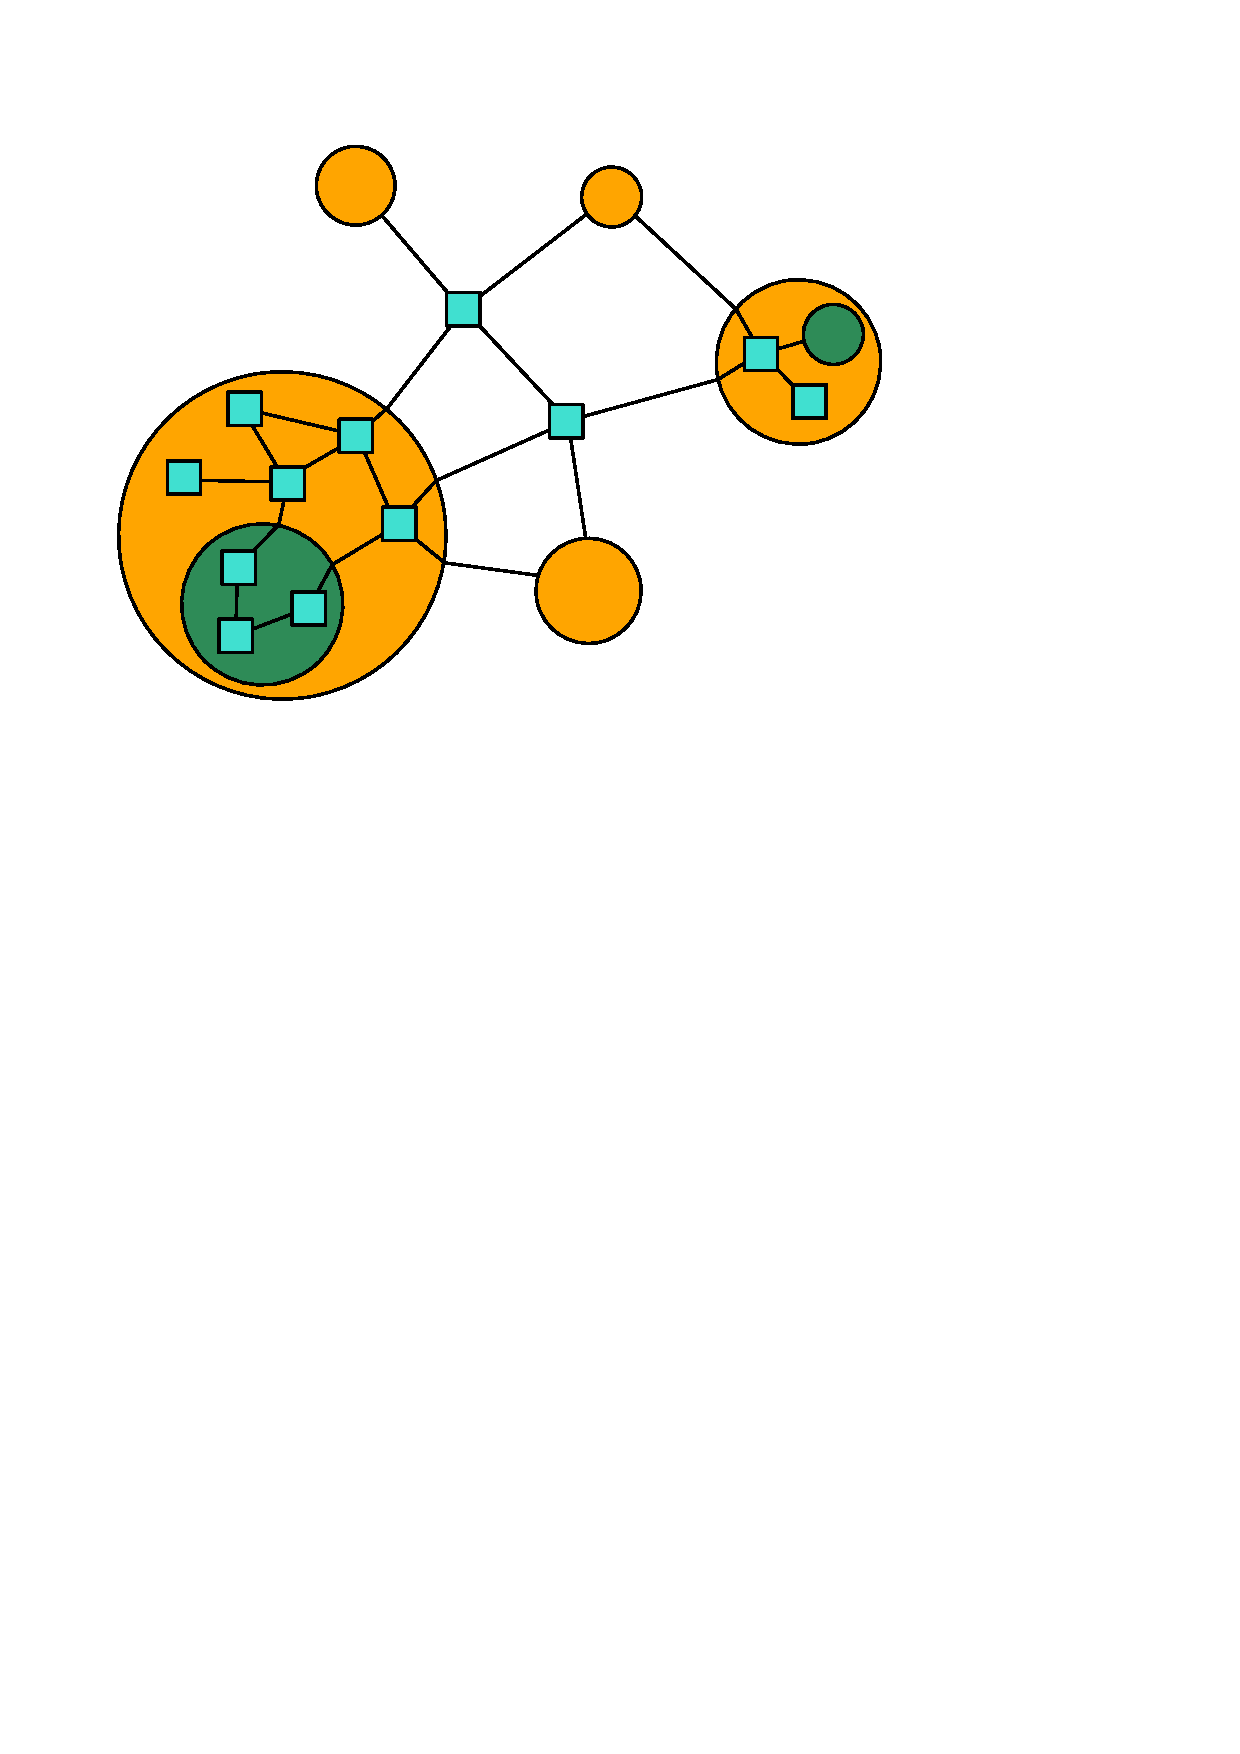
\includegraphics[width=0.7\linewidth]{Pics/Layoutbeispiel.pdf}
  \caption{Beispiellayout einer abstrahierten Argumentkarte nach unserem Konzept.}
  \label{f:Layoutbeispiel}
\end{center}
\end{figure}

% welche Schritte?
Im Folgenden beschreiben wir  in \autoref{sec:Algo} einen Algorithmus um so ein Layout zu berechnen, 
sowie in \autoref{sec:Interaktion} das Konzept um Layoutänderungen bei Interaktionen mit Gruppen gering zu halten.
Zunächst widmen wir uns jedoch kräftebasierten Algorithmen, die wir für unsere Ansätze benutzen, sowie der Größe von geschlossenen Gruppen im Layout.

\myparagraph{Kräftebasierter Algorithmus}
Grundlage für unseren Algorithmus ist die Verwendung eines kräftebasierten Algorithmus. Als Kräfte haben wir unter anderemr die Anziehung adjazenter Knoten bzw. Gruppen,
die Abstoßung zwischen nicht-adjazenten Knoten bzw. Gruppen, sowie die Abstoßung von Knoten selbst, sodass keine adjazenten Elemente die nicht punktförmigen Knoten oder Gruppen schneiden. Außerdem wird eine Abstoßung zwischen Kanten und nicht-inzidenten Knoten bzw. Gruppen benötigt, um Knoten-Kanten-Überschneidungen zu verhindern.
Zusätzlich benötigen wir sogenannte Anker, welche einzelnen Knoten oder Gruppen zugeordnet werden. 
Ein Anker ist ein Pseudoknoten, welcher  nich gerendert wird, sowie eine Kante zu seinem Knoten. 
Anders als normale Kanten ist die optimale Kantenlänge eines Ankers  0. Außerdem ist die Position des Ankers im Layout fest. 
In einem kräftebasierten Algorithmus wirkt der Anker auf seinen Knoten nun wie eine weitere Feder, die ihn zum Ankerpunkt hinzieht.
Die Kraft der Feder kann wie eine normale Kante gehandhabt werden oder bei Bedarf auch anders spezifiziert werden.
Als Grundlage für diesen kräftebasieren Algorithmus könnten man zum Beispiel der Algorithmus von Fruchterman und Reingold \cite{SPE:SPE4380211102} verwenden werden.
Mit nicht punktförmigen Knoten hat sich zum Beispiel bereits Harel und Koren \cite{Harel:2002:DGN:1556262.1556288} beschäftigt.


% Größe geschlossener Gruppen
\myparagraph{Gruppengrößen}
Wie die Größe einer geöffneten Gruppe berechnet werden kann ist in einem späteren Abschnitt genauer beschrieben. 
Eine jedoch vom beschriebenen Algorithmus unabhängige Designentscheidung ist die Größe von geschlossenen Gruppen.
Während eine Möglichkeit wäre, jede geschlossen Gruppe mit einem gleich großen Kreis darzustellen, schlagen wir einen anderen Ansatz vor.

Um direkt zu sehen, ob sich hinter einer geschlossenen Gruppe eine große oder kleine Gruppe bzw. eine mit vielen oder wenigen Kindelemente befindet, empfiehlt es sich den Kreisradius der geschlossenen Gruppe in Beziehung zu der Anzahl der Kindelemente sowie der Größe der Gruppe im offenen Zustand zu setzen.
Da die Größe einer offenen Gruppe stark mit den Anzahl der Kindelemente korreliert, wird dadurch auch diese Eigenschaft einer Gruppe durch die geschlossene Repräsentation
wiedergegeben.
Die Größe der geschlossenen Gruppe könnte also dadurch berechnet werden, dass sie auf einer Skala von einer minimalen bis zu einer maximalen Größe abgebildet wird.
Die minimale Größe könnte hierbei zum Beispiel durch die Größe des am größten dargstellten Arguments gegeben sein und die maximale Größe durch $\gamma \,\%$ 
der größten Gruppe im geöffneten Zustand.

Da der Unterschied zwischen kleinen Gruppen, wobei zum Beispiel eine 4 Kindelemente Besitzt und einer etwas größere die 5 besitzt, stärker verdeutlicht werden soll, als der zwischen 
relativ großen Gruppen, schlagen wir eine logarithmische Abbildung wie in \autoref{f:Radius} vor.
\begin{figure}[h!]
\begin{center} 
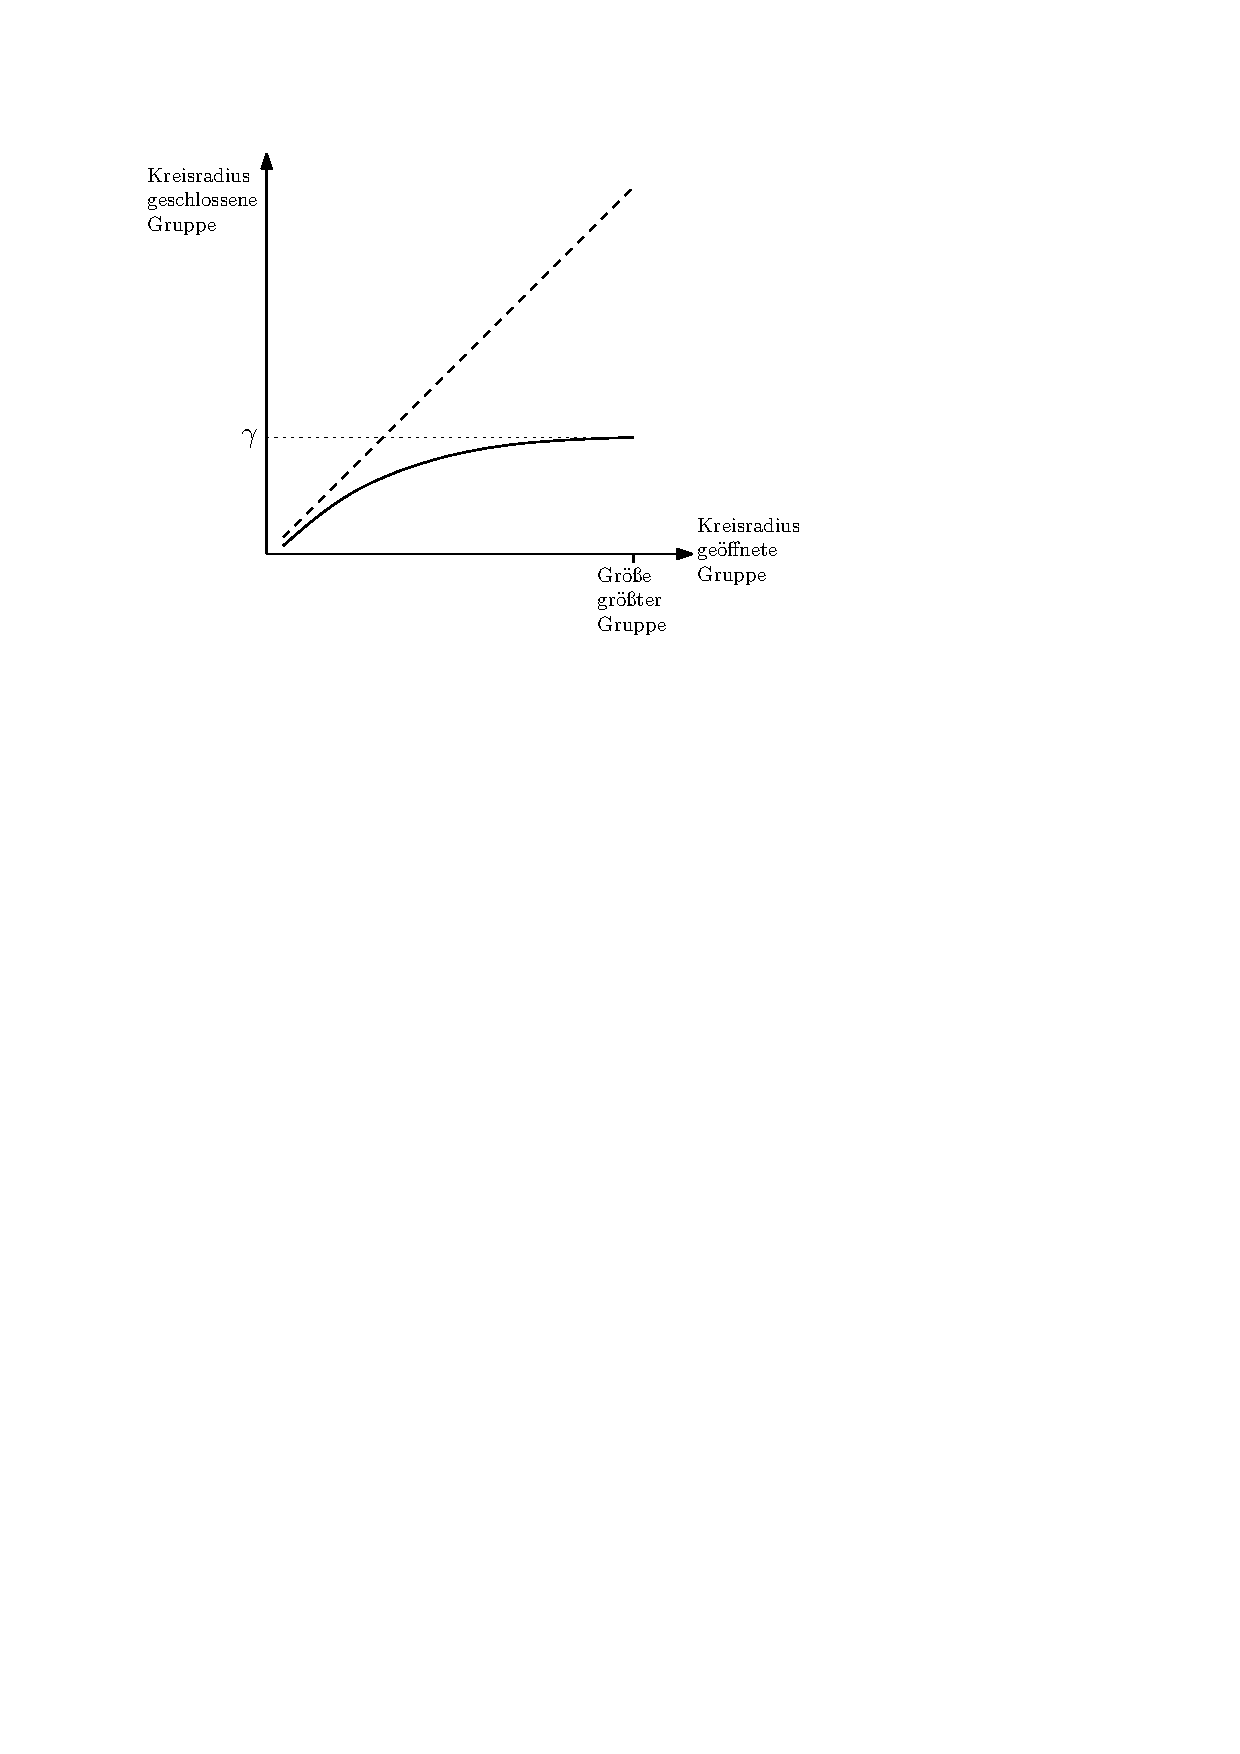
\includegraphics{Pics/Radius.pdf}
% 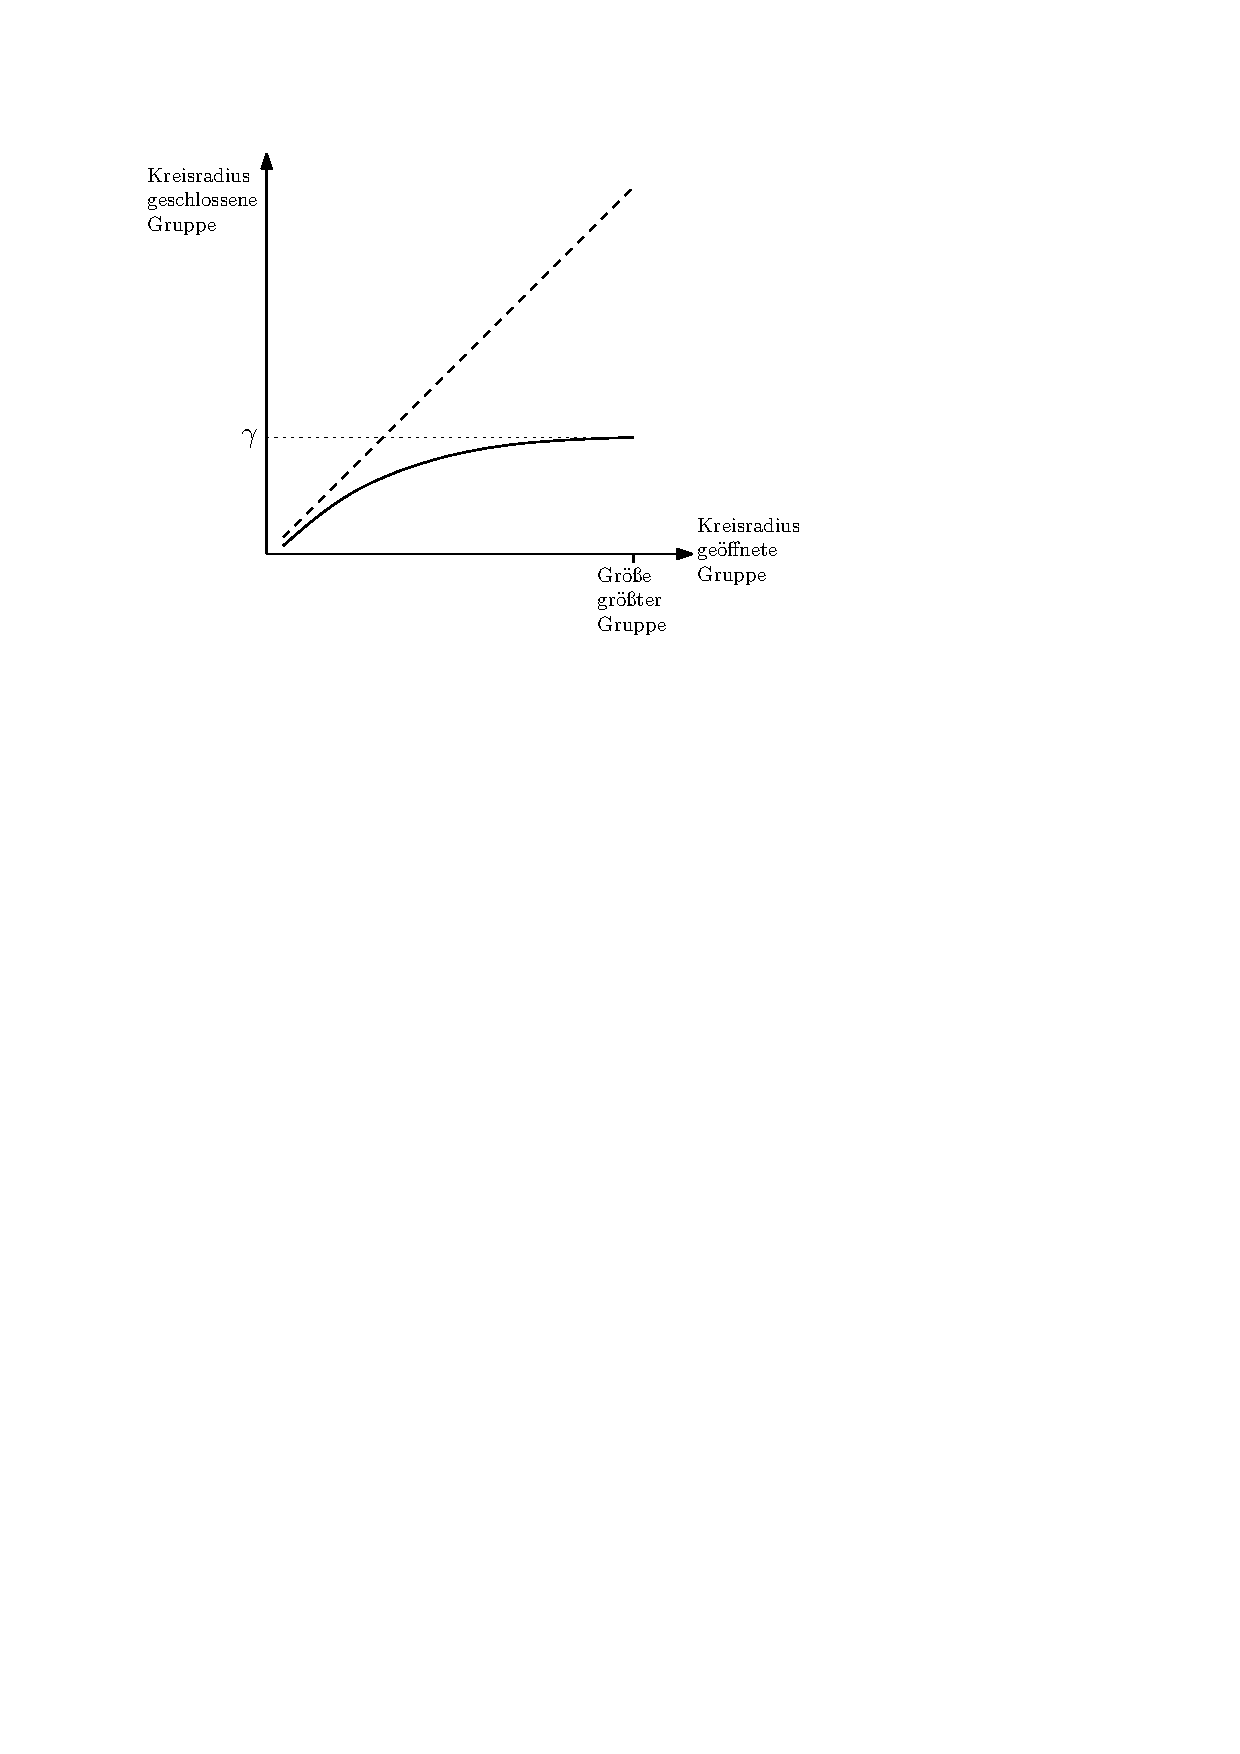
\includegraphics[width=0.5\textwidth]{Pics/Radius.pdf}
  \caption{Vorgeschlagene Wahl der Gruppengröße einer geschlossenen Gruppe in Abhängigkeit der Gruppe in geöffnetem Zustand. }
  \label{f:Radius}
\end{center}
\end{figure}
%\todo[inline]{Gamma Wert weglassen}


\section{Konzept und Idee}
\label{sec:Algo}
% Weitere Constraints für Layout
% Resultat: alle Gruppen geschlossen, jedoch Layout pro Gruppe mit geschlossenen/geöffneten Kind-Gruppen bekannt
Wenn alle Gruppen beim Öffnen einer Karte geschlossen sind, sollte es auf großen Karten einfach sein direkt einen Überblick gewinnen zu können.
Deshalb liefert der folgendes Algorithmus ein Layout bei dem initial alle Gruppen geschlossen sind.

Unser in \autoref{Layoutalgorithmus} grob beschriebene Layoutalgorithmus ist in 2 Phasen unterteilt. 
In der ersten Phase, Zeilen 1-9, werden die in einem bottem-up Ansatz die Größen der Gruppen und erste Layout $\L'$ berechnet. 
Dies beginnt auf der tiefsten Stufe und geht dann iterativ nach oben, da die Größe einer Gruppe jeweils für die Größe der übergordneten Gruppe bzw. obersten Stufe notwendig ist.
In einem top-down Ansatz werden in der zweiten Phase, Zeilen 10-18, nun die Layouts pro Stufe und Gruppe $\L_H$ berechnet und die Ports festgelegt. Das gesamte Layout setzt 
sich dann aus dem Layout der obersten Stufe und den Layouts pro Gruppe zusammen.

\begin{algorithm}[H]
\label{Layoutalgorithmus}
\SetAlgoLined
\Ein{Graph $G=(V,E)$,  Gruppenbaum $T$ } % mit Koten $V$ mit Größe, gerichteten \& gefärbten Kanten $E$, Mengen $S$ von Knoten und Elementen aus $S$
\Aus{Gruppen-hierarchisches Layout von $G$ } % mit diesen und jenen Eigenschaften, evtl Name einführen für Referenzierung
$i =$ niedrigste Stufe einer Gruppe\;
\Solange{$i < höchste Stufe$}{ 
  \Fuer{Jede Gruppe $H$ auf Stufe $i$} {
	berechnete Layout $\L'_H$ der Gruppe $H$\;
	berechne benötigte Fläche des Gruppenlayouts\;	
  }
  $i= i + 1$\;
}
Berechne Layout auf höchster Stufe\;
Lege Ports für Gruppen auf der zweithöchsten Stufe fest\;
$i =$ zweithöchste Stufe\; 
\Solange{$i \geq$ niedrigste Stufe}{ %Anzahl Stufen % benötigt, dass oberste Ebene auch Gruppe
  \Fuer{Jede Gruppe $H$ auf Stufe $i$} {
	berechnete Layout $\L_H$ der Gruppe $H$ unter Berücksichtigung der Ports\;
	Lege Ports für Gruppen in $H$ auf Stufe $i + 1$ fest;
  }
  $i= i - 1$\;
}
\caption{Layoutalgorithmus}
\end{algorithm}
%\todo[inline]{Algo ist korrigiert muss aber korrekturgelesen werden <- erst Formales klären, Stufen definieren, dann anpassen!}

Im Folgenden beschreiben wir den bottom-up und den top-down Anteil des Algorithmus genauer. 

\subsection{Bottom-up Anteil des Algorithmus}
Schauen wir uns den bottom-up Anteil des Algorithmus genauer an. Ziel ist es zunächst für jede Gruppe ein benötigte Größe zu approximieren.
Da für die Gruppen die Positionen der Ports jedoch noch nicht bekannt sind, werden die Gruppen zunächst ohne Ports gelayoutet.
Hierfür verwenden wir den oben beschrieben kräftebasierten Algorithmus. 
Zusätzlich wird  für jeden Knoten noch ein Anker zu einer relativen Mitte der Gruppe gesetzt. 
Auf Grund der Verwendung eines kräftebasierten Algorithmus hält dies die Gruppe, die nicht zwingend eine Zusammenhangskomponente sein muss, zusammen 
und konzentriert sie in einem eher kreisförmigen Bereich. Anderenfalls könnte sich zum Beispiel eine lange Kette bilden.

Da die Größe von Kindgruppen einer Elterngruppe für deren Layout benötigt wird, beginnt der Algorithmus auf der tiefsten Stufe,
also bei den Gruppen, die in den meisten Gruppen enthalten sind. Wurde ein Layout berechnet, kann ein Kreis darum gelegt werden und somit die Größe approximiert werden.
Mit der oben genannten Rechnung für die Größe von geschlossenen Gruppen, kann nun also die Größe für das Layout eine Stufe höher verwendet werden.
Dies wiederholt sich bis zur obersten Stufe. Hier sind jedoch keine Anker zu einem Mittelpunkt mehr zwingend nötig.
Dies ist nur der Fall, wenn man die gesamte Karte  in einen keisförmigen Bereich ziehen möchte.

\begin{figure}[h!]
\begin{center} 
  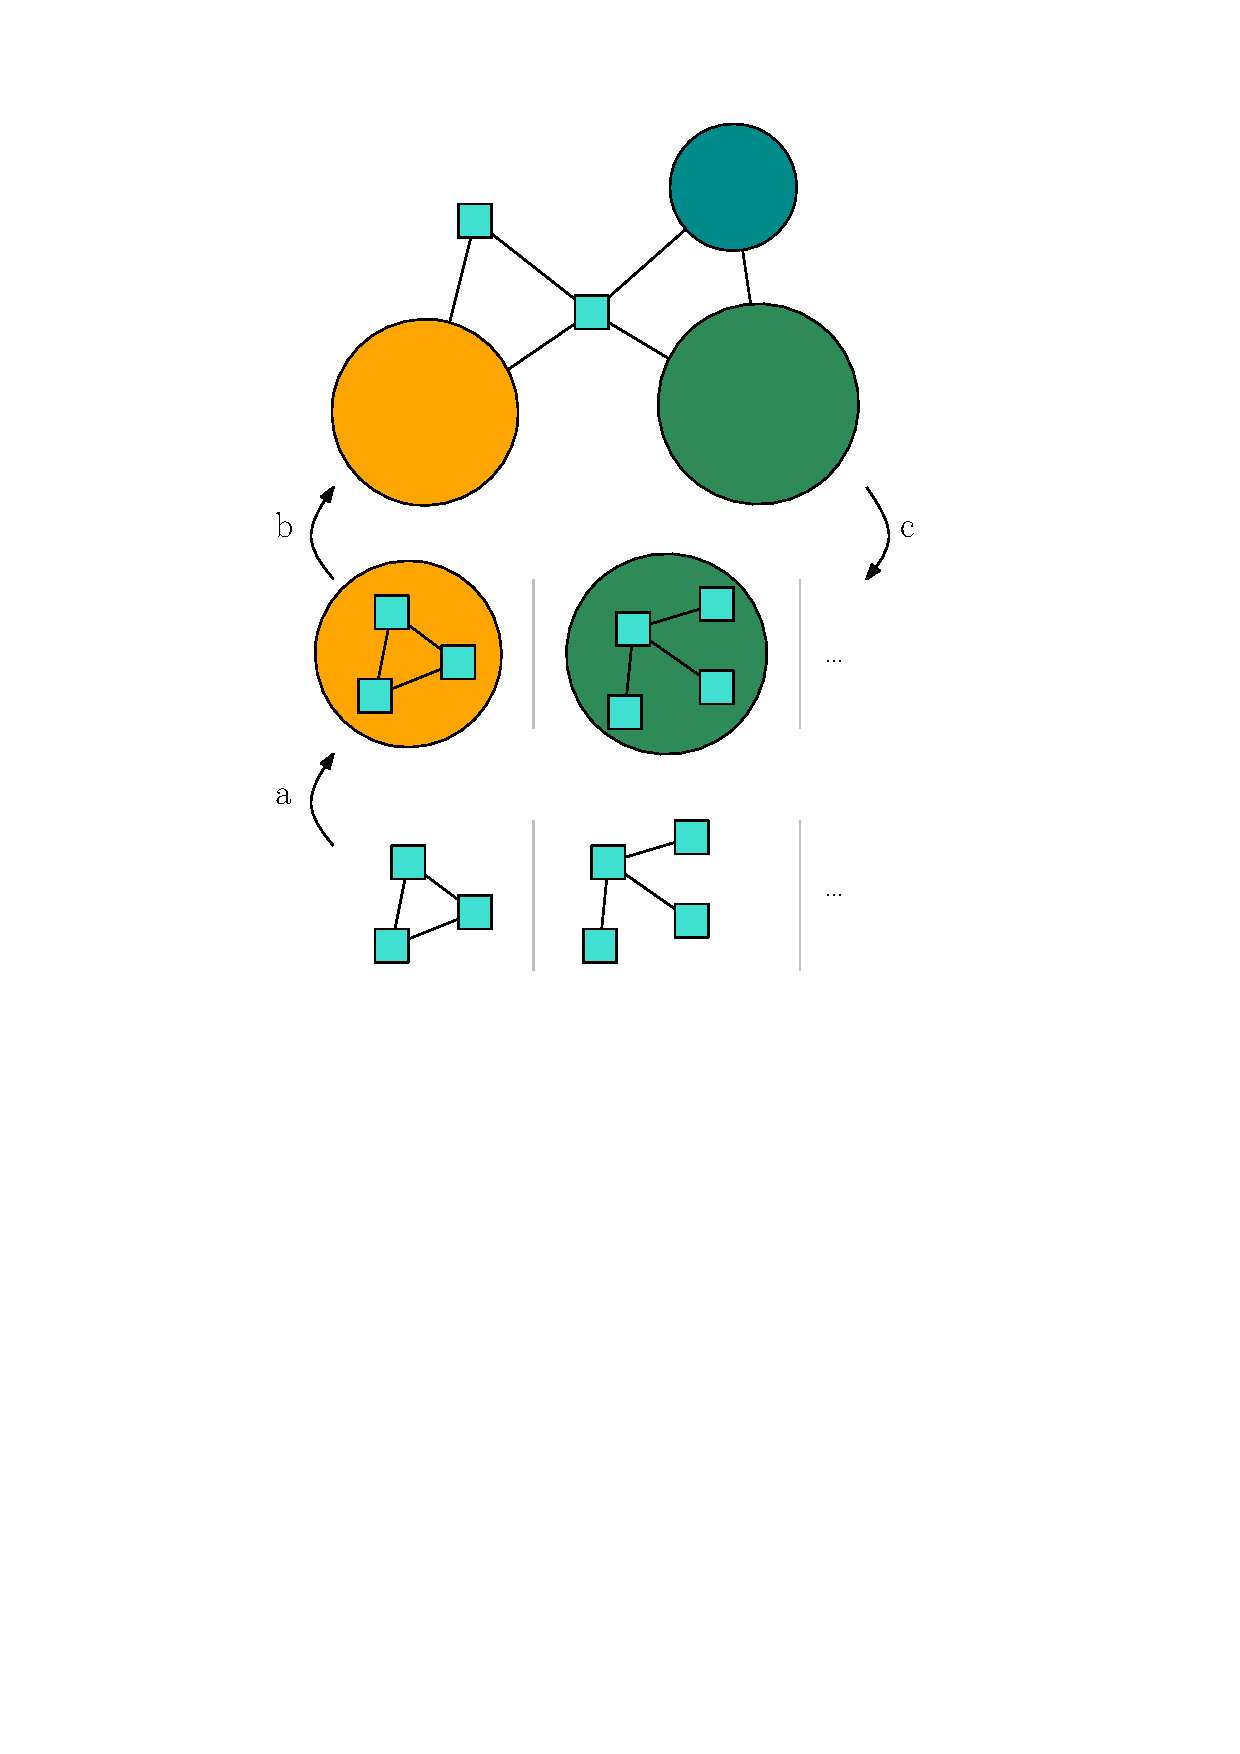
\includegraphics[width=0.5\textwidth]{Pics/BottomUp2.pdf}
  \caption{Bottom-up Anteil des Algorithmus zur Berechnung der benötigten Größen.
  Nachdem Layouts auf der untersten Stufe berechnet wurden (Zeile 4, \autoref{Layoutalgorithmus}) wir in Schritt $a$ die benötigt Größe der Gruppe berechnet (Zeile 5). 
  Nun kann dieser Prozess mit $b$ und $c$ bis zur obersten Stufe wiederholt werden. }
  \label{f:BottomUp}
\end{center}
\end{figure}


\subsection{Top-down Anteil des Algorithmus}
Der Übergang vom bottom-up zum top-down Anteil erfolgt, wenn in Zeile 9 auf der obersten Stufe das Layout berechnet wird.
Wenn zu Beginn, wie bei uns gewählt, alle Gruppen geschlossen sind, dann ist dieses berechnete Layout auch das Layout, das beim Öffnen der Karte zu sehen ist.
Auf der obersten Stufe beginnend und durch das berechnete Layout vorgegeben, legen wir nun die Ports der Gruppen der darunterliegenden Stufe fest und berechnen deren Layouts.

\begin{figure}[h!]
\begin{center} 
  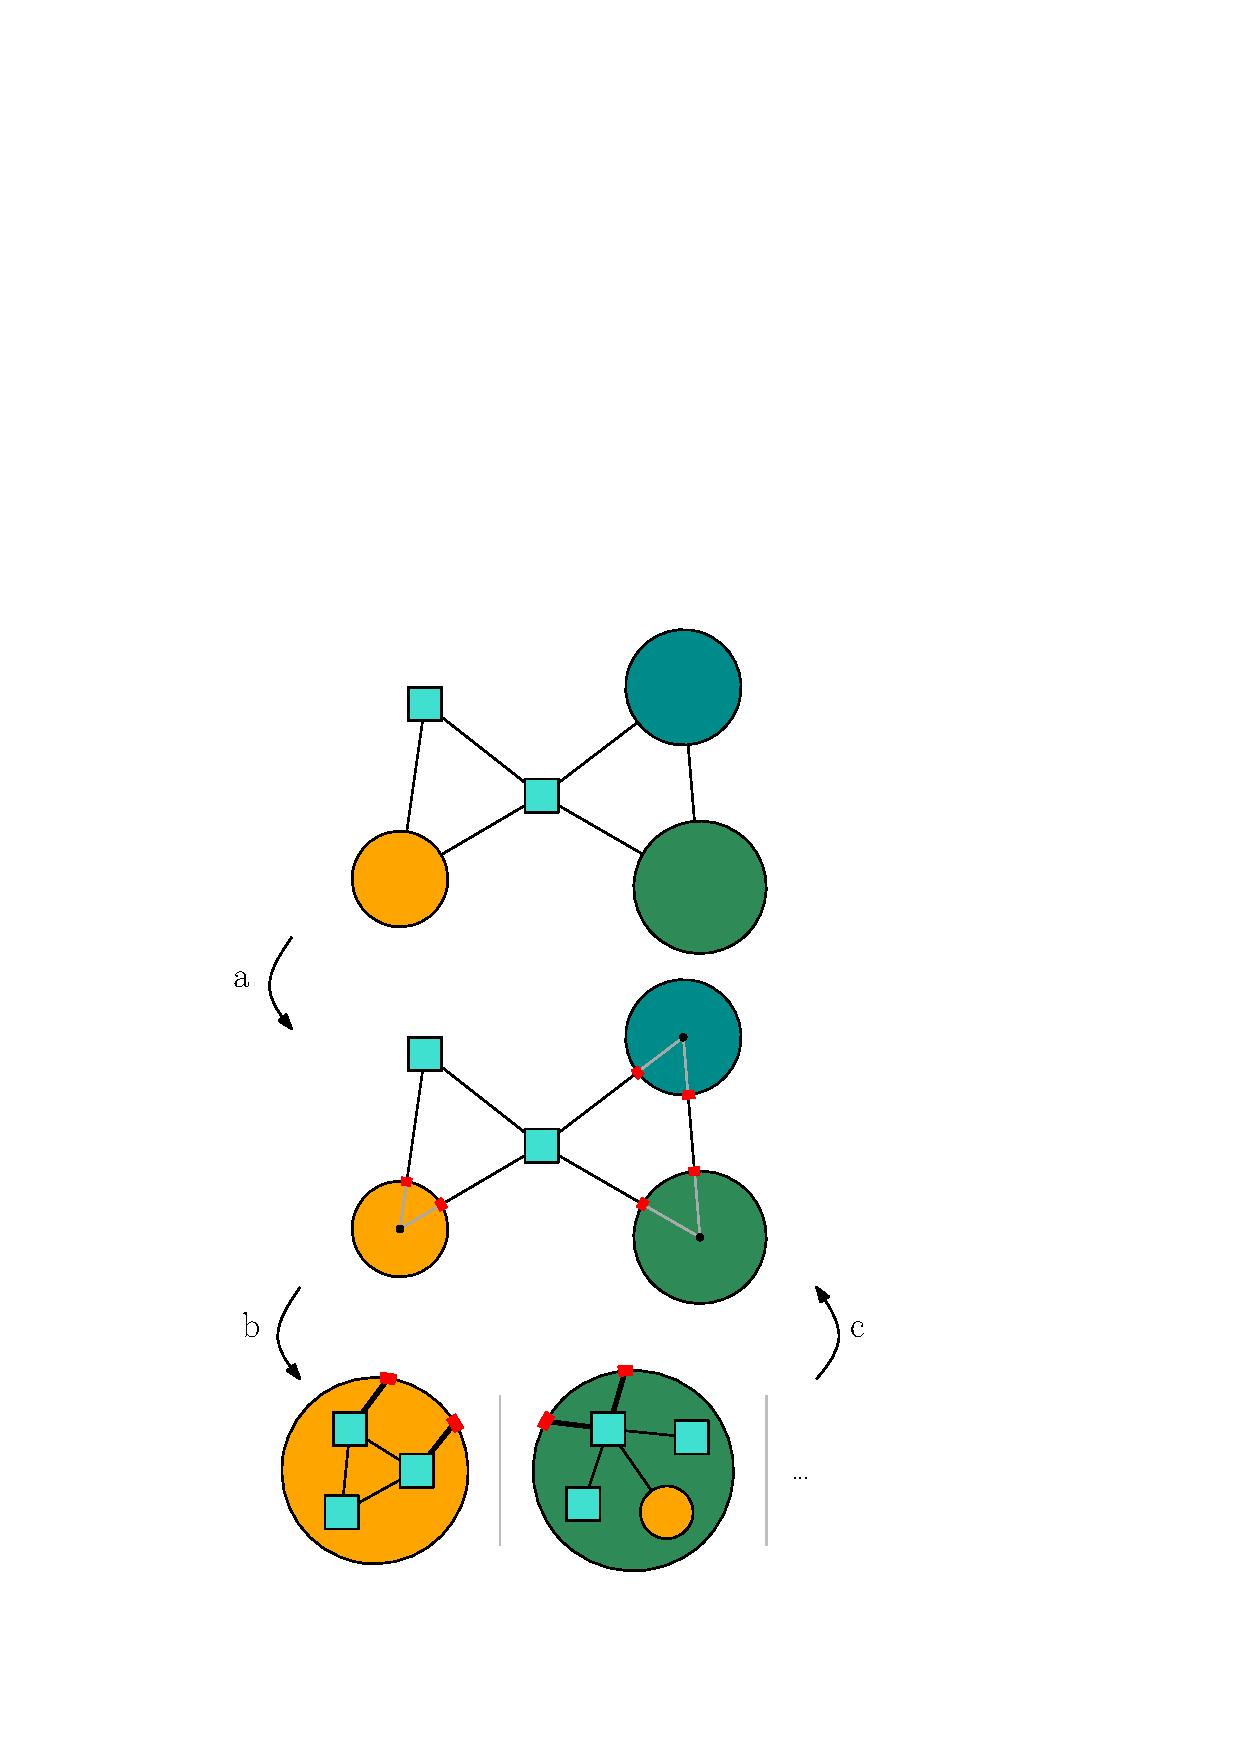
\includegraphics[width=0.5\textwidth]{Pics/TopDown.pdf}
  \caption{Top-down Anteil des Algorithmus zur Festlegung der Ports und Berechnung der Layouts.
  Mit dem Layout der höchsten Stufe können in Schritt $a$ die Ports für die niedrigere Stufe berechnet werden (Zeile 9, \autoref{Layoutalgorithmus}).
  In Schritt $b$ wird dann das Layout der nächsten Stufe mit Ports berechnet (Zeile 13).
  Dieser Prozess mit $b$ und $c$ bis zur untersten Stufe wiederholt werden. }
  \label{f:TopDown}
\end{center}
\end{figure}


%\subsubsection*{Layout in Gruppen in Abhängigkeit von Ports}
% Problem: Layout eines Graphens (mit Labelknoten) innerhalb eines Kreises mit Ports für ausgehende kanten
% Äquivalent: Layout eines Graphens mit punktförmigen Knoten auf Kreis und gelabelten Knoten innerhalb des Kreises
% was betrachten?
Im Folgenden betrachten wir nun die Zeilen 14 und 15 des \hyperref[Layoutalgorithmus]{Layoutalgorithmus~\ref*{Layoutalgorithmus}} genauer. 
% was ist ziel?
Hier ist das Ziel ein Layout für eine Gruppe in Abhängigkeit von bereits gegebenen Ports zu finden, sowie daraufhin dessen Kindgruppen Ports zuzuweisen.
Das heißt, wir suchen nun ein Layout für die Kindknoten einer Gruppe sowie aus der Gruppe herausgehende Kanten.
Dieses soll, wie oben beschrieben, ein Layout innerhalb eines Kreises sein und die Gruppengrenze-überschreitenden Kanten zu den festgelegten Ports führen.
% was ist schwierig?
Eine der Herausforderung hierbei ist, eine geeignete Größe für den Kreis um die Gruppe zu finden. 
Auch zum Finden dieses Layouts benutzen wir wieder den kräftebasierten Algorithmus.

Das bestimmen der Ports ist einfach umzusetzen. 
Wenn ein Layout berechnet wird, werden die Kanten zu einer Gruppe so gelayoutet, dass sie eine inzidente Gruppe nur radial schneiden.
Der erhaltene Schnittpunkt mit dem Kreis der Gruppe legt so die Position für den Port fest, welche einfach durch den Winkel beschrieben werden kann. 
Dies ist auch in Abbildung \autoref{f:TopDown} dargestellt.
Da davon auszugehen ist, dass sich bei Veränderungen im Layout die Winkel nicht zu sehr ändern werden, bleiben die Winkel für jede Gruppengröße fest.
Dadurch bleibt das Layout in einer Gruppe unabhängig von den Änderungen außerhalb. 
Jedoch müssen die verschiedenen Ansätze für das Kantenrouting im verwendeten Algorithmus für die Interaktion beachtet werden.

Für die Layoutberechnung ist eine Gruppe $H$, sowie die vom Layouts der darüberliegenden Stufe bereits festgelegten Ports der Gruppe gegeben.
Diese Ports modellieren wir als feste Knoten auf dem Kreis der Gruppe an ihren jeweiligen Winkeln.
Des Weiteren haben wir bereits ein Layout $\mathcal{L_H}$ der Gruppe $H$ ohne Gruppengrenze-überschreitenden Kanten in Zeile 4 des \hyperref[Layoutalgorithmus]{Layoutalgorithmus~\ref*{Layoutalgorithmus}}  berechnet. 
Aus Zeile 5 haben wir daher auch eine erste Größe für den Kreis der Gruppe, welche durch den Radius beschreiben und durch $R'_H$ gegeben sei. 

Der grobe Ablauf des Algorithmus setzt sich aus drei Schritten zusammen. Zunächst wird ein Anfangslayouts gewählt.
Dann wird ein optimaler Radius  berechnet sowie das Layout berechnet. 
Die Wahl eines Anfangslayouts und das Finden eines optimalen Radius beschrieben wir in den folgenden Abschnitten genauer. 

%\begin{algorithm}[H]
%\label{Gruppenlayoutalgorithmus}
%\SetAlgoLined
%\Ein{Gruppe $H$, sowie Ports und Kanten zu Ports} 
%\Aus{Gruppenlayout $\L_H$ von $H$ }
%Wähle Anfangslayout\;
%Finde Radius $R$ für Kreis\;
%Berechne Gruppenlayout  $\L_H$ mit kräftebasiertem Algorithmus\;
%\caption{Gruppenlayoutalgorithmus}
%\end{algorithm}

Für die Berechnung eines Gruppenlayouts verwenden wir wieder den oben geforderten kräftebasierten Algorithmus, welcher mit Knoten von bestimmter Größer umgehen kann. 
Jedoch schlagen wir auch hier wieder das Hinzunehmen eines Ankers vor, welcher alle Elemente zur Mitte des Kreises ziehen soll.
Dies soll auch verhindern, dass eventuell nicht zusammenhängende Komponenten der Gruppe auseinander driften. 
Die Kraft dieses Ankers sei mit dem Faktor $\alpha$ beschrieben. 
Solange der Kreis der Gruppe groß genug ist, sollte es für Knoten auch nicht möglich sein, aus dem Kreis herausgetragen zu werden. 
Andernfalls müssten man hierfür weitere Kräfte im Algorithmus berücksichtigen oder $\alpha$ entsprechend erhöhen.

% - Anfangslayout: 
\myparagraph{Anfangslayout}
Für die Wahl eines Anfangslayouts schlagen wir folgenden Ansatz vor.
	% c) Layout von Größenberechnung spiegeln (nicht, vertikal, horizontal, beides) und Längen der Port-Knoten-Kanten summieren
In Zeile 4 von \autoref{Layoutalgorithmus} wurde für $H$ bereits ein Layout $\L'_H$ berechnet. 
Dieses lässt sich sowohl horizontal als auch vertikal spiegeln, ohne die Ausrichtung der einzelnen Knoten, welche nach den Achsen ausgerichtete Rechtecke sind, verändert wird.
Das heißt, wir haben vier verschiedene Layouts, nämlich das original, das vertikal oder horizontal gespiegelte sowie das vertikal und horizontal gespiegelte.
Um lange Kanten von Knoten zu Ports durch die ganze Gruppe möglichst zu vermeiden, wählen wir jenes Layout,
bei dem die Summe der Kantenlängen dieser Kanten am kleinsten ist. Dies ist das gewählte Anfangslayout $\mathcal{L}'_H$.
\autoref{f:Anfangslayout} gibt hierfür ein Beispiel.

\begin{figure}[h!]
\begin{center} 
  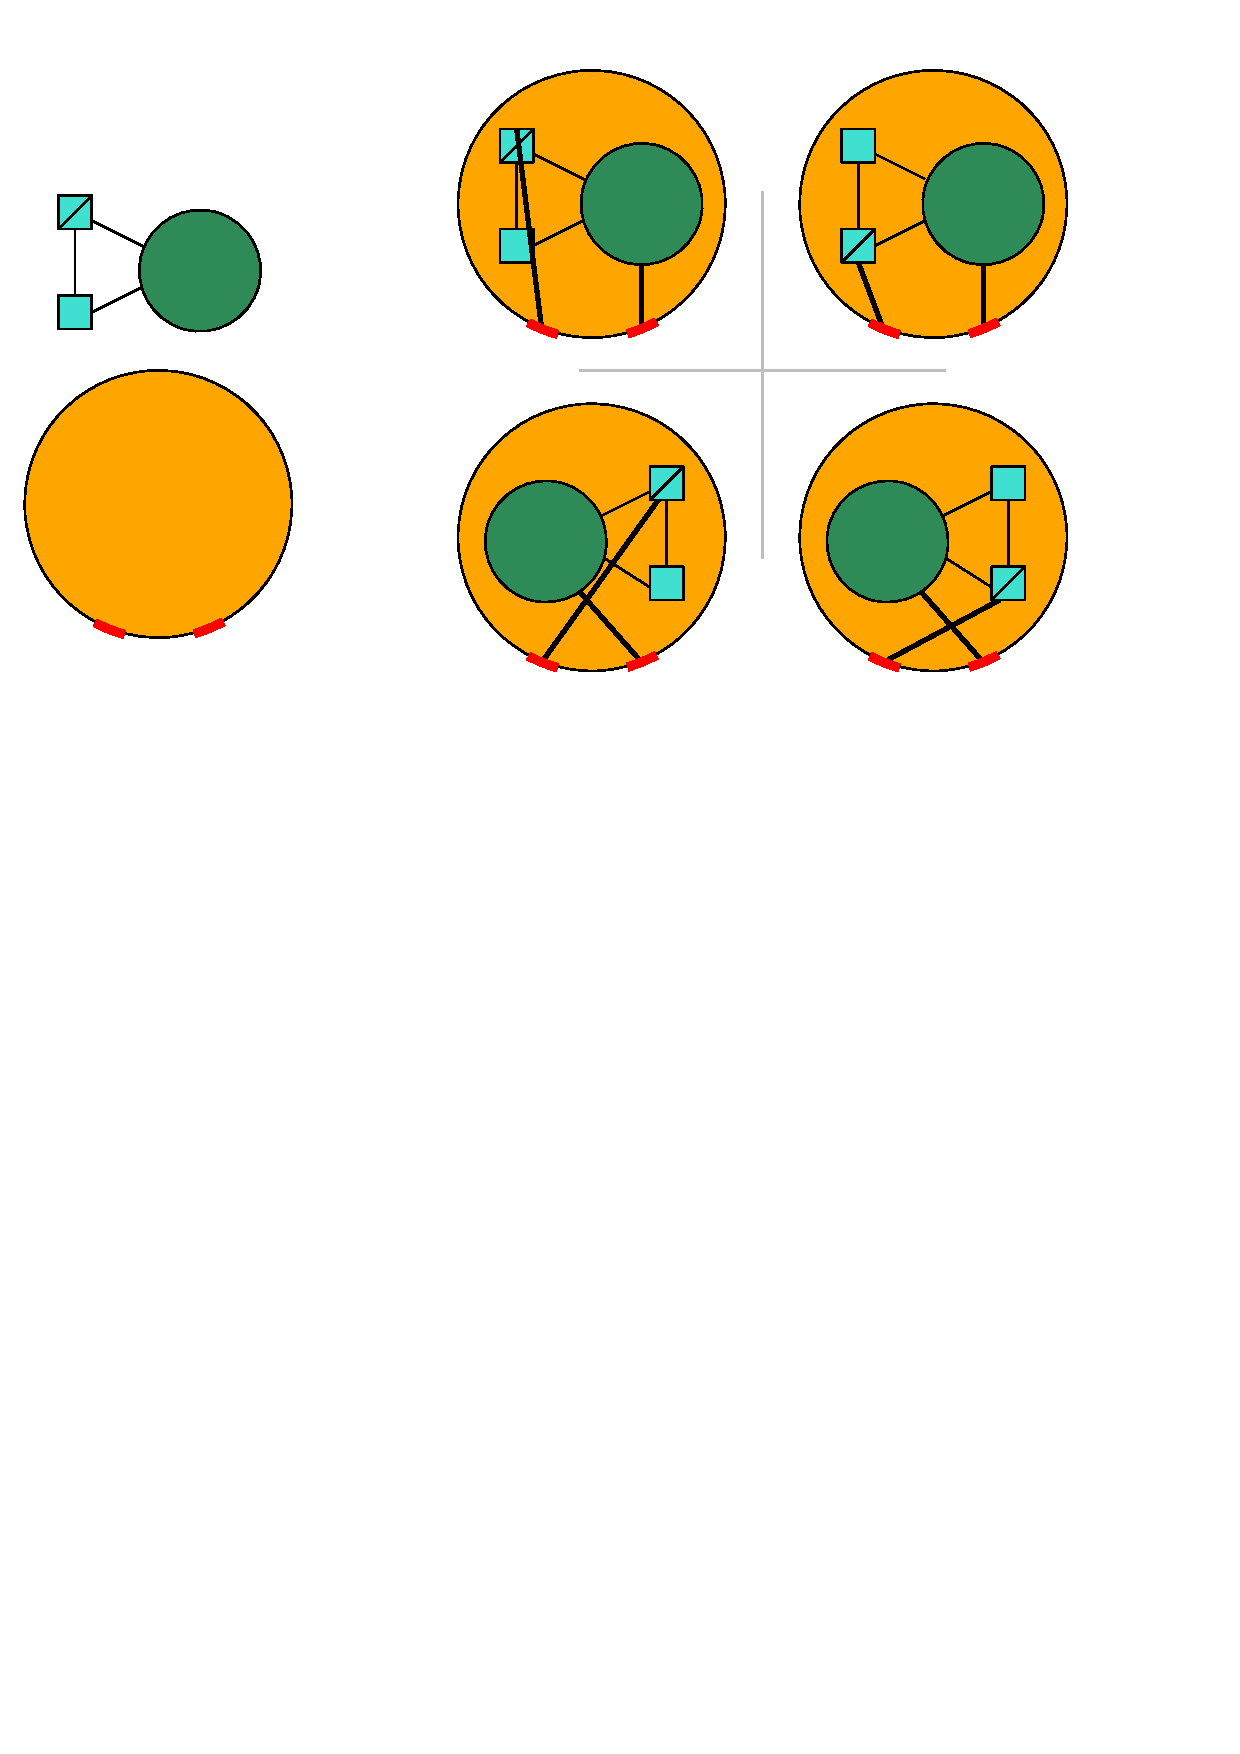
\includegraphics[width=0.8\textwidth]{Pics/Anfangslayout.pdf}
  \caption{Ansatz zur Wahl des Anfangslayouts. Links das vorberechnete innere Layout und die Elterngruppe mit Ports. Rechts die vier verschiedene Spiegelungen des Layouts sowie die Kanten zu den Ports.
  In diesem Fall würde das rechte obere, also horizontal gespiegelte, Layout als Anfangslayout gewählt werden, da die Gesamtlänge der Kanten zu den Ports hier am kürzesten ist.}
  \label{f:Anfangslayout}
\end{center}
\end{figure}

Natürlich gibt es  noch weitere Ansätze zum Finden eines Anfangslayouts.
Einfache Ansätze wären zum Beispiel eine zufällige Platzierung der Knoten oder die Platzierung aller Knoten in die Mitte des Kreises, 
um dann den Rest dem kräftebasierten Layoutalgorithmus zu überlassen. 
Man könnte sich jedoch auch einen anspruchsvolleren Ansatz überlegen, bei dem man das Gruppenlayout ausgehend von den Ports konstruiert.

Mit gewähltem Anfangslayout können wir nun den optimalen Kreisradius einer Gruppe bestimmen.

% - Größe des Kreises definiert durch Radius R
\myparagraph{Bestimmen des Kreisradius einer geöffneten Gruppe}
Für die Berechnung eines angemessenen Kreisradius schlagen wir einen iterativen Algorithmus vor. \label{Radius}
Hierbei führen wir die beiden Schritte Finden des Radius und Berechnen des Layouts zusammen aus.
Die Idee des iterativen Algorithmus ist es, für einen gegeben Radius ein Layout zu berechnen und dann zu testen, ob der Radius verkleinert werden kann.
Ist dies der Fall, so wiederhole das Vorgehen. Ansonsten erhöhe entweder den Faktor $\alpha$ für die Kraft des Ankers zum Mittelpunkt oder breche ab. 
Da hier noch die Anfangsberechnung der Layouts in Gruppen beschreiben wird, ist es wichtig anzumerken, dass die Kindggruppen der behandelten Gruppe 
geschlossen % wieso?
sind.
Wird der Algorithmus später verwendet, muss dies nicht mehr der Fall sein.
\todo[inline]{Wieso geöffnet? Nicht geschlossen sinnvoler? Bei Änderung nachschauen ob oben wo so erwähnt.}

Als Anfangsradius des Algorithmus kann der Radius $R'_H$ aus \autoref{Layoutalgorithmus} Zeile 5 mal einem Faktor $\beta$ verwendet werden.
Die Wahl des Anfangslayouts haben wir im Abschnitt davor beschrieben.

\begin{algorithm}[H]
\label{Kreisradiusalgorithmus}
\SetAlgoLined
\Ein{Gruppe $H$, Ports, Kanten zu Ports, Anfangslayout $\L'_H$, Radius $R'_H$}
\Aus{Gruppenlayout $\L_H$ von $H$, Radius $R_H$}
$R = \beta \cdot R'_H = $ Anfangsradius für Kreis\;
$\L_H = \L'_H \cup$ Ports $\cup$  Kanten zu Ports\;
Führe kräftebasiertem Algorithmus auf  $L_H$ aus\;
\eWenn{$R$ verkleinert werden kann}{
	Passe $R$ an\;
}{
	\eWenn{$\alpha$ nicht zu groß}{
		erhöhe $\alpha$\;
		gehe zu 3\;
	}{
		Algorithmus fertig\;
	}
}
\caption{Kreisradiusalgorithmus}
\end{algorithm}

Für \autoref{Kreisradiusalgorithmus} muss natürlich noch spezifiziert werden, was es heißt, dass der Radius in Zeile 4 verkleinert werden kann
oder dass $\alpha$ nicht zu groß ist. 
Dass der Radius $R$ verkleinert werden kann, soll bedeuten, dass bei kleinerem $R$ aber gleichem Layout der Kreis keine Knoten schneidet. 
Typisch für Parameter bei kräftebasierten Algorithmen, wird um eine geeignete maximale Größe von $\alpha$ zu finden, wohl eine Implementierung und verschiedene Tests benötigt. 
Dasselbe gilt für $\beta$ um einen geeigeneten Anfangsradius zu finden.

Eine weitere Variante zur Berechnung des Kreisradius könnte durch erwartete Größe von Gruppen umgesetzt werden. 
Falls ein gutes $\beta$ gefunden werden kann, dass für jede Gruppe eine gute Größe approximiert und dabei nie zu klein ist, kann der iterative Prozess auch ausgelassen werden
und der Radius der Gruppe für jeden Zustand direkt berechnet werden.			

% Anmerkung: Da in Praxis (Argumentkarten) die Gruppentiefe nicht hoch ist und in Gruppe nicht viele Gruppen sind, 
			% können hier auch die Größen für alle Fälle berechnet werden
% Postprocessing: Kantenklätung

Abschließend zur Beschreibung der Layoutberechnung wollen wir anmerken, dass die bottom-up und top-down Anteile auch wiederholt durchgeführt werden können.
Dadurch können die benötigten Größen in den Layoutberechnungen besser berücksichtigt werden und so auch die resultierende Ports besser festgelegt werden.

%---------------------------------------------------------------------------------------------
\section{Layout-Anpassung bei Interaktion}%statt: m Öffnen oder Schließen einer Gruppe}
% was betrachten?
\label{sec:Interaktion}
Nachdem ein Anfangslayout für die ganze Argumentkarte gefunden wurde, bei der alle Gruppen geschlossen sind, möchte man nun auch Gruppen öffnen. 
Das Layout für jede Gruppe wurde ebenfalls bereits berechnet. Zur Erinnerung, wenn eine Gruppe geschlossen ist, hat sie eine Größe, 
die Abhängig von der Größe im offenen Zustand kleiner ist. 
Da diese Gruppe im geöffneten Zustand nun jedoch mehr Platz einnimmt ergibt sich folgende Problemstellung:
% was ist ziel?
Wie verändert sich das Layout auf darüberligenden Stufen, wenn eine Gruppe geöffnet oder geschlossen wird? 
Hierbei wird wie spezifiert außerdem gefordert, dass die Änderungen im Layout nicht zu stark sind, 
damit man sich mit seiner mentalen Karte von vor der Änderung auch danach noch zurechtfindet.
% was ist schwierig?

Der von uns vorgeschlagene Lösungsansatz basiert erneut auf einem kräftebasierten Algorithmus. 
Auch hier verweisen wir auf den oben beschriebenen Algorithmus. Es gibt zwei Probleme zu lösen. 
Zum Einen, wie groß ist eine Gruppe in ihrem jetzigen Zustand.  
Zum Anderen, wie man dafür sorgt, dass sich das Layout nach Öffnen oder Schließen einer Gruppe nicht zu sehr verändert.

% Ansatz für Größe
Um die Größe einer Gruppe in ihrem jetzigen Zustand zu berechnen, könnte man verschieden vorgehen. 
Zum Beispiel könnte man ihn aus den bekannten Radien, für den Zustand alle Untergruppen geöffnet und der Gruppe selbst geschlossen, berechnen. 
Oder aber man benutzt den Algorithmus aus dem vorherigen Abschnitt, um ihn entweder im Vorraus oder wenn benötigt zu ermitteln. 
Wird nun eine Gruppe geöffnet oder geschlossen, wird diese durch eine größere bzw. kleinere ersetzt. 
Diese Änderung zieht sich logischer Weise bis zur obersten Stufe durch.

Um das Verhalten bei einer Interkation mit einer Gruppe zu kontrollieren, erweitern wir den verwendeten kräftebasierten Layoutalgorithmus um mehrere Anker. 
Dies geschieht pro Stufe und Gruppe für die ein neues Layout berechnet werden muss.
Jedes gelayoutet Element, was sich also nicht in einer geschlossenen Gruppe befindet, bekommt einen Anker gesetzt und zwar an der Position, 
an der es sich im Anfangslayout der Gruppe bzw. obersten Stufe befindet. 
Diese Anker bezeichnen wir als Grundanker. 
Wenn nun eine Gruppe geöffnet oder geschlossen wird und die dadurch verursachten Größenänderungen pro Stufe durchgeführt wurden, 
wird in jeder veränderten Gruppe sowie der obersten Stufe der Layoutalgorithmus mit den zuvor gesetzten Grundankern gestartet. 
Dies wird  durch \autoref{f:Interaktion} veranschaulicht. 
Die Grundanker sorgen nur dafür, dass die Elemente nicht zu stark von ihrer Position vor der Veränderung verschoben werden.

\begin{figure}[h!]
\begin{center} 
  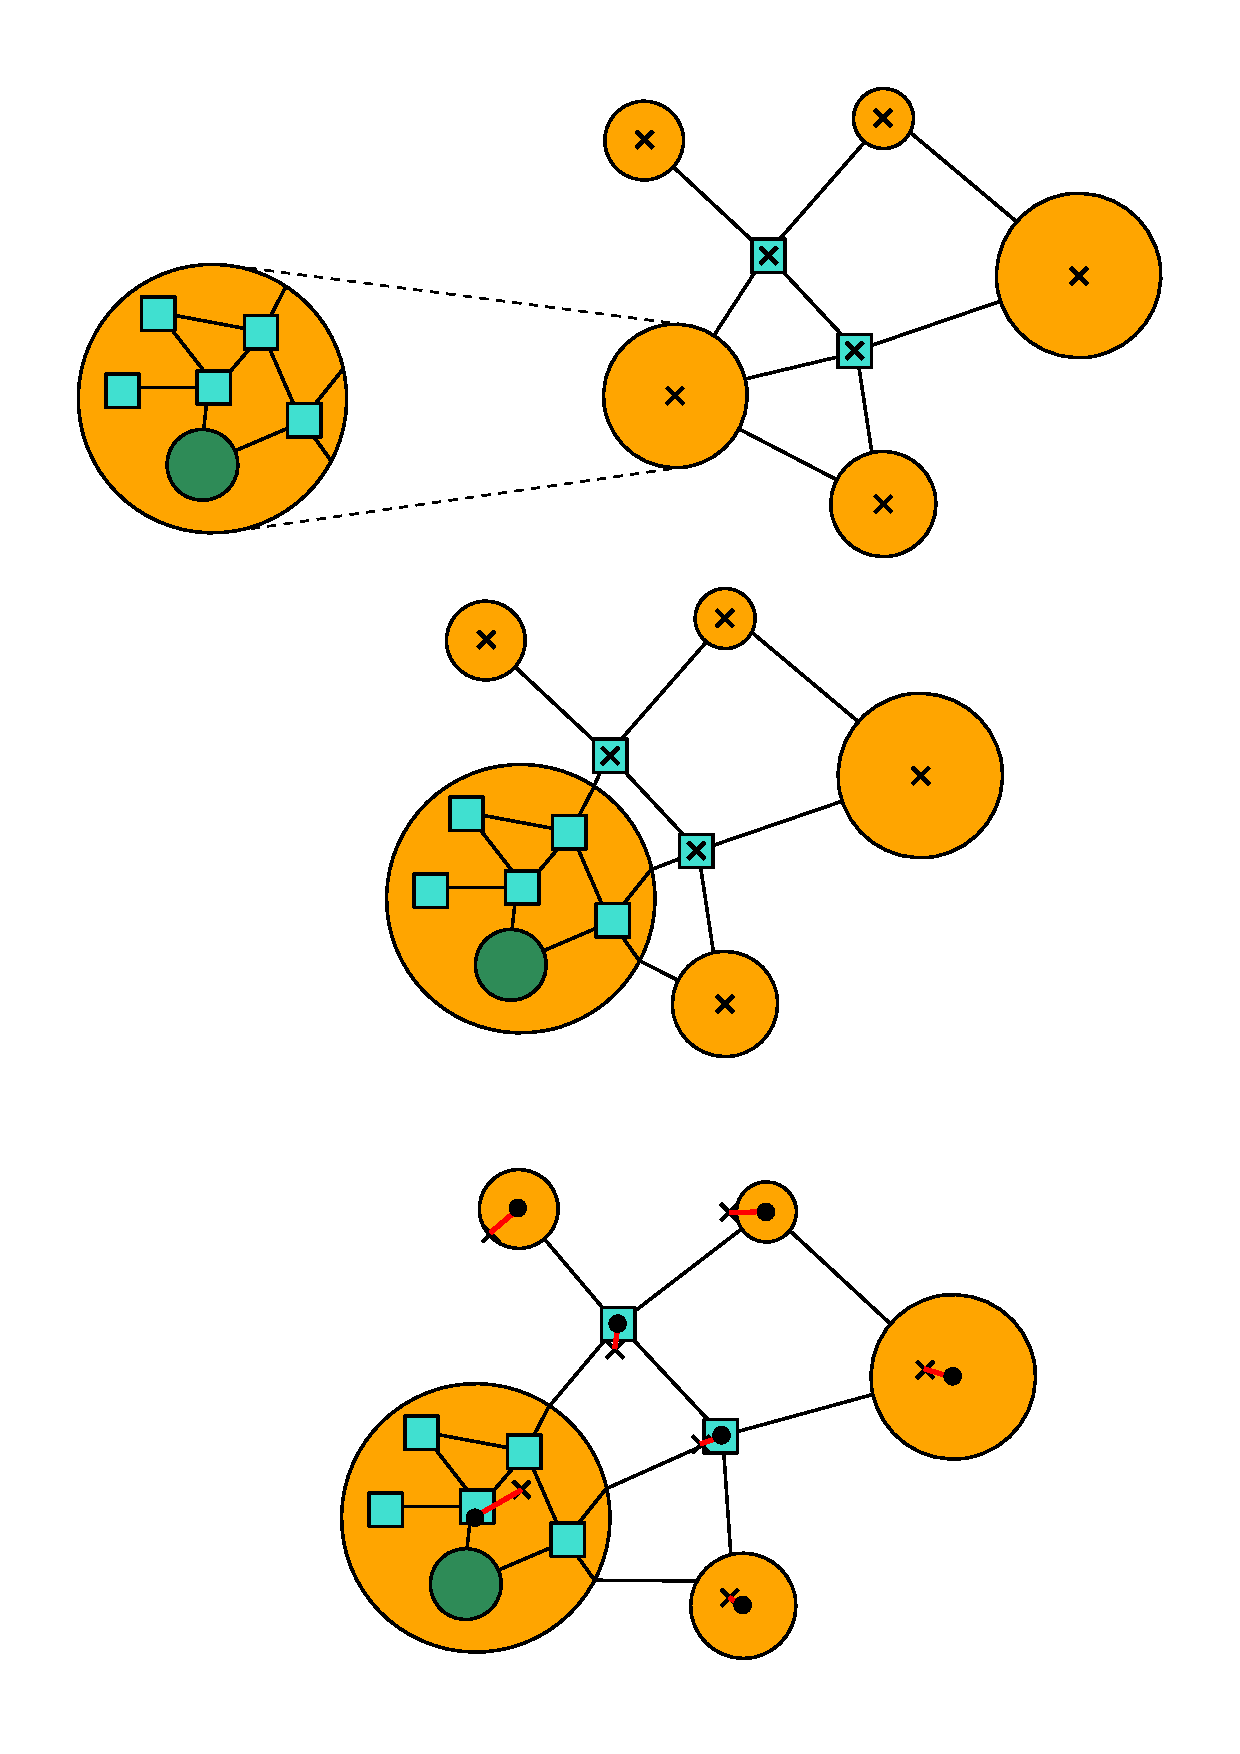
\includegraphics[width=0.7\textwidth]{Pics/Interaktion.pdf}
  \caption{Veranschaulichung des Ankerprinzips beim Öffnen einer Gruppe.}
  \label{f:Interaktion}
\end{center}
\end{figure}

Genauer zu spezifizieren ist, wie stark die Anker sein sollten sowie ob sie von der Gruppen- bzw. Elementgröße abhängig sein sollten. 
Hierfür sind erneut eine Implementierung sowie Tests nötig. Dies Wahl könnte natürlich auch sehr von der Argumentkartenstruktur sowie der eigenen Vorliebe abhängen.

Durch das Öffnen vieler Gruppen können große Veränderungen zum Grundlayout zustande kommen.
Die Kräfte der Anker könnten so im Verhältnis zu anderen Kräften zu stark werden und unschöne Layouts erzeugen.
Deshalb ist ein weiterer Punkt bei diesem Lösungsansatz, dass in einem solchen Fall die Grundanker ignoriert werden 
und lediglich temporär neue Anker vor der letzten Änderung gesetzt werden. 
Es wird also nur versucht zum letzten Layout die Veränderungen gering zu erhalten, nicht jedoch direkt zum Anfangslayouts. 
Wann dieser Fall eintritt muss noch genauer spezifiert werden und kann pro Stufe unterschiedlich gehandhabt werden.

% ------- Vorgehen für Parameterwahl vorschlagen
%\todo[inline]{Vorgehen für Parameterwahl vorschlagen?}
